\chapter{Tensor Calculus}\label{cap:6}
\section{Partial Derivative of a Tensor}\label{sec:6.1}
In the last chapter, we met algebraic operations which are tensorial, that is, which convert tensors into tensors. The operations are addition, subtraction, multiplication, and contraction. The next question which arises is, What differential operations are there that are tensorial? The answer to this turns out to be very much more envolced. The first thing we shall see is the partial differentations of tensors is \textbf{not} tensorial. Different authors denote the partial derivative of a contravariant vector $X^{a}$ by $$\partial_bX^{a}\quad \mbox{or} \quad \pdv{X^{a}}{x^b}\quad\mbox{or}\quad \tensor{X}{^{a}_{,b}} \quad \mbox{or}\quad \tensor{X}{^{a}_{|b}}$$
and similarly for higher-rank tensors. We shall use a mixture of all the first three notations. (Note that in the literature, the partial derivative of a tensor is often referred to ad the \textbf{ordinary} derivativa of a tensor, to distinguish ir from the tensorial differentiation we shall shortly meet). Now differentiating (\ref{5.16}) with respect to $x'^c$, we find
\begin{align}
	\nonumber\partial '_xX'^{a}&=\frac{\partial}{\partial x'^c}\left(\pdv{x'^{a}}{x^b}X^b\right)\\
					\nonumber					&=\pdv{x^d}{x'^c}\frac{\partial}{\partial x^d}\left(\pdv{x'^{a}}{x^b}X^b\right)\\
														&=\pdv{x'^{a}}{x^b}\pdv{x^d}{x'^c}\partial _dX^b+\frac{\partial^2x'^{a}}{\partial x^b\partial x^d}\pdv{x^d}{x'^c}X^b\label{6.1}
\end{align}
If the first term on the right-hand side alone were present, then this would be the usual tensor transformation law of a tensor of type $(1,1)$. However, the presence of the second term prevents $\partial_bX^{a}$ from behaving like a tensor.

There is a fundamental reason why this is the case. By definition, the process of differentiation involves comparing a quantity evaluated at two neighboring points, $P$ and $Q$ say, dividing by some parameter representing the separation of $P$ and $Q$ and then taking the limit as this parameter goes to zero. In the case of a cintravariant vector field $X^{a}$, this would involve computing $$\lim_{\delta u\to 0}\frac{[X^{a}]_P-[X^{a}]_Q}{\delta u}$$ for some appropiate parameter $\delta u$. However, from the transformation law in the form (\ref{5.25}), we see that $$X'^{a}_P=\left[\pdv{x'^{a}}{x^b}\right]_PX^b_P\quad\mbox{and}\quad X'^{a}_Q=\left[\pdv{x'^{a}}{x^b}\right]_QX^b_Q$$ This involves the transformation matrix evaluated at \textbf{differnet} points, from which it should be clear that $X^{a}_P - X^{a}_P$ is not a tensor. Similar remarks hold for differentiating tensors in general.

It turns out that if  we wish to differentiate a tensor in a tensorial manner then we need to introduce some auxiliary field into the manifold. We shall meet three different types of diffenrentiation. First of all, in the next section, we shall introduce a \textbf{contravariant vector field} onto the manifold and ise it to define the \textbf{Lie derivative}. Then we shall introduce a quantity called an \textbf{afine connection} and use it to define \textbf{covariant differentiation}. Finally, we shall introduce a tensor called a \textbf{metric} and from it build a special affine conection, called the \textbf{metric connection}, and again define \textbf{covariant differentiation} but relative to this specific connection.

\section{The Lie Derivative}\label{sec:6.2}
The argument we present in this section is rather intricate. It rest on the idea of interpreting a coordinate transformation \textbf{actively} as a point transformation, rather that \textbf{passively} as we have done up to now.  The important results occur at the end of the section and consist of the formula for the Lie derivative of a general tensor fields and the basic properties of Lie differentiation.

We start by considering a \textbf{cogurence of curves}  defined such that inly one curve goes through each point in the manifold. Then, given any one curce of the congruence, $$x^{a}=x^{a}(u),$$ we can ise it to define the tangent vector field $\dd x^{a}/\dd u$ along the curve. If we do this for every curve in the congruence, then we end up with a vector field $X^{a}$ (given $\dv*{x^{a}}{u}$ at each point) defined over the whole manifold. 

Conversely, given a non-zero vector field $X^{a}(x)$ defined over the manifold, then this can be used to define a congruence of curves in the manifold called the \textbf{orbits} or \textbf{trajectories} of $X^{a}$. The procedure is exactly the same as the way in which a vector field gives rise to field lines or streamlines in vector analysis. These curves are obtained by solving the ordinary diffrerentual equations
\begin{equation}\label{6.2}
	\pdv{x^{a}}{u}=X^{a}(x(u))
\end{equation}
The existence and uniqueness theorem for ordinary differnetial equations guarantees a solution, at least for some subset of the reals. In what follows, we are really only interested in what happens locally.

We therefore assume that $X^{a}$ has been given and we have constructed the local congruence of curves. Suppose we have some tensor fields $T^{a\cdots}_{b\cdots}(x)$ which we wish to differentiate using $X^{a}$. Thene the essential idea is to use the congruence of curves to \textbf{drag} the tensor at some point $P$ (i.e. $T^{a\cdots}_{b\cdots}(x)$) along the curve passing through $P$ to some neighbouring point $Q$, and then compare this "dragged-along tensor" with the tensor already there (i.e. $T^{a\cdots}_{b\cdots}(Q)$) (Fig \ref{fig:6.3}). Since the dragged-along tensor will be of the same type as the tensor already at $Q$, we can \textbf{subtract the two tensors at $Q$} and so define a derivative by some limiting process as $Q$ tends to $P$. The technique for dragging involves viewing the coordinate transformation from $P$ to $Q$ \textbf{actively}, and applying it to the usual tranformation law of tensors. We shall consider the detailed calculation in the case of a contravariant tensor field of rank $2$, $T{ab}(x)$ say.

\begin{figure}[h!]
	\begin{center}
		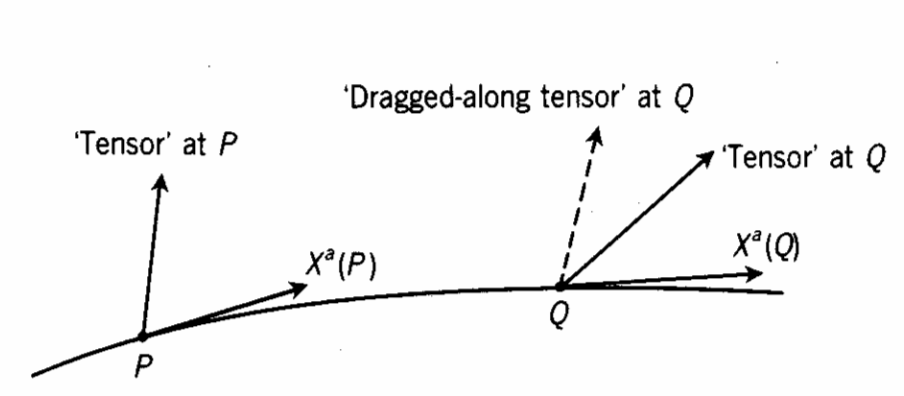
\includegraphics[scale=0.5]{fig/fig:6-3.png}
		\caption{Using the congruence to compare tensors at neighbouring points.}
		\label{fig:6.3}
	\end{center}	
\end{figure}

Consider the transformation
\begin{equation}\label{6.3}\marginnote{Point transformation}
	\boxed{x'^{a}=x^{a}+\delta u X^{a}(x)}
\end{equation}
where $\delta u$ is small. This is called a \textbf{point transformation} and is to be regarded actively as sending the point $P$, with cooridantes $x^{a}$, to the point $Q$, with coordinates $x^{a}+\delta uX^{a}(x)$, where the coordinates of each point are given in the \textbf{same} $x^{a}$-coordinae system, i.e.
\begin{align*}
	P&\to Q\\
	x^{a}&\to x^{a}+\delta uX^{a}(x)
\end{align*}





